\subsection{Probability Distribution}
With an understanding of parameters, we can now move on to distributions. Data can come in various distributions depending on different parameters such
as degrees of freedom. The distribution is the shape of the data and it will have
an effect on statistical models. Therefore it is important to have an understanding of distributions.
\subsubsection{Normal Distribution}

In the world of statistics, the most common distribution is the normal distribution, it's called the bell shape. The normal distribution is a continuous distribution, with this density function:

\begin{equation}
n(x;\mu,\sigma) =\frac{1}{\sqrt{2\pi\sigma}}e^{-\frac{(x-\mu)}{2\sigma^2}}
\end{equation}

\noindent The distribution is dependent on the mean($\mu$) and the standard deviation($\sigma$), where changes to the mean will result in a change in the positioning of the normal distribution. Whereas a change in the standard deviation will change the spread of the curve. The normal distribution also always contains an area under the curve that is equal to one. This is to ensure that the normal distribution correctly models probability. There is a special variation of the normal distribution, called the standard normal distribution, where the mean is zero and the standard deviation is one. The standard normal distribution can be seen in \autoref{fig:Norm}, this distribution is widely used in statistics as it makes math behind computing statistical inference easier.
\begin{figure}[h!]
	\centering
	\begin{minipage}{0.80\textwidth}
		\centering
		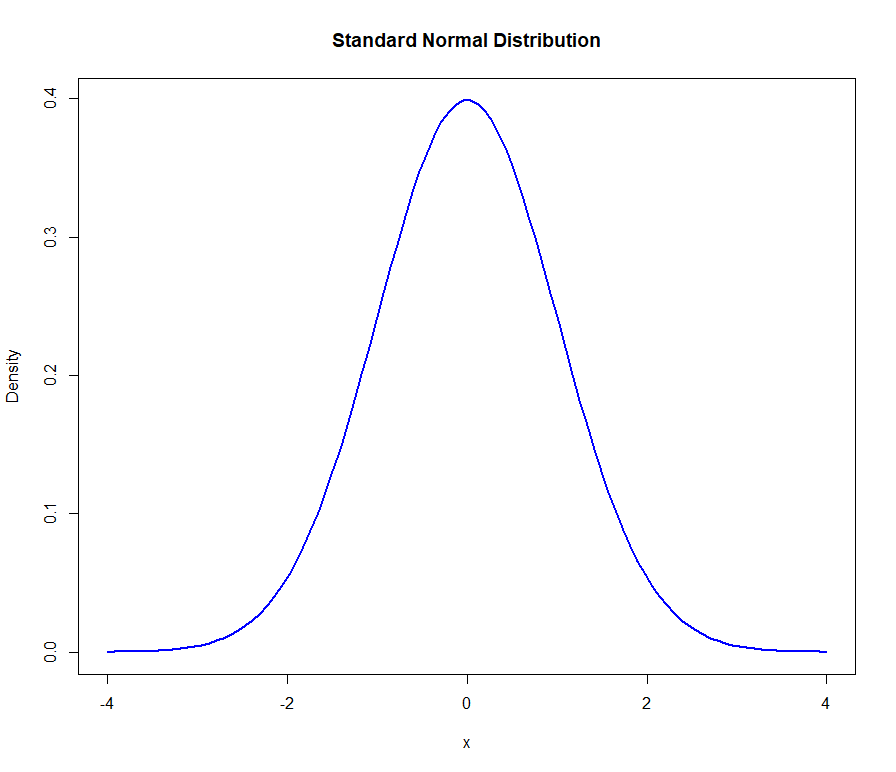
\includegraphics[width=\linewidth]{billder/Normal distribution.png}
		\caption{The standard normal distribution}
		\label{fig:Norm}
	\end{minipage}\hfill
\end{figure}
All variations of a normal distribution can be standardized by a transformation of the distribution, using the Z-score formula.
\newline
\begin{equation}
Z=\frac{X-\mu}{\sigma}
\end{equation}


\noindent $Z$ in the Z-score represents the amount of standard deviations a given $X$ value, deviates from the mean.

\subsubsection{The Central Limit Theorem}
A very effective theorem in statistics is the central limit theorem. This theorem states that if a random sample $\overline{X}$, with the size $n$, is taken from a population with a mean and a finite variance, then as $n$ goes towards infinity, the distribution will resemble a normal distribution. If used with the Z-score formula, the distribution will resemble a standard normal distribution. The formula for the Z-score, when in conjunction with the central limit theorem, looks like this:

\begin{equation}
Z=\frac{\overline{X}-\mu}{\sigma/\sqrt{n}}
\end{equation}


\noindent Where $\bar{X}$ is a random sample of size $n$ and $\mu$ is the mean of the true population. The standard error i represented by $\sigma/\sqrt{n}$, where $\sigma$ is the standard deviation and $n$ is the sample size.
Usually the standard deviation is unknown, for these situations it's possible to use the estimator $S^2$. This estimates the variance of the population from the variance of the sample, by this formula:

\begin{equation}
s^2=\sum_{i=1}^{n}\frac{(x_{i}-\bar{x})}{n-1}
\end{equation}
The square root of the variance is the standard deviation, therefore the square root of the estimator $S^2$ would be the estimated standard deviation. The problem with using the estimator $S^2$, is that with small samples the variance is small and therefore it contains a lot of bias. In this situation the t-distribution would be used instead of the normal distribution, because the t-distribution takes the bias into account the bias of the standard deviation. It does this by having thicker tails, meaning that the probability of more extreme values are higher.

\subsubsection{The t-Distribution}
The t-distribution is shaped as the standard normal distribution, in a bell shape and symmetrical around the mean of zero, the difference is that the t-distribution contains more variance. This comes from the fact that the t-distribution is dependent on the degrees of freedom. When the degrees of freedom surpasses 30, the rule of thumb is that the distribution will resemble a normal distribution. So before 30 degrees of freedom, the distribution contains more variance.
The t-distribution will come to resemble the standard normal distribution, when in surpasses 30 degrees of freedom, this makes sense, since the two distributions have the same formula:
\begin{equation}
	T=\frac{\bar{X}-\mu}{S/\sqrt{n}}
\end{equation}
The only difference is the estimated standard deviation $S$.
As seen in \autoref{fig:t-dist}, the t-distribution approaches the normal distribution as the degrees of freedom increases. The t-distribution with a smaller amount of degrees of freedom, will have more mass further out from the center, but as the degrees of freedom increases and approaches 30, then the mass will shift towards the center and shaping itself as the standard normal distribution.
\begin{figure}[h!]
	\centering
	\begin{minipage}{0.80\textwidth}
		\centering
		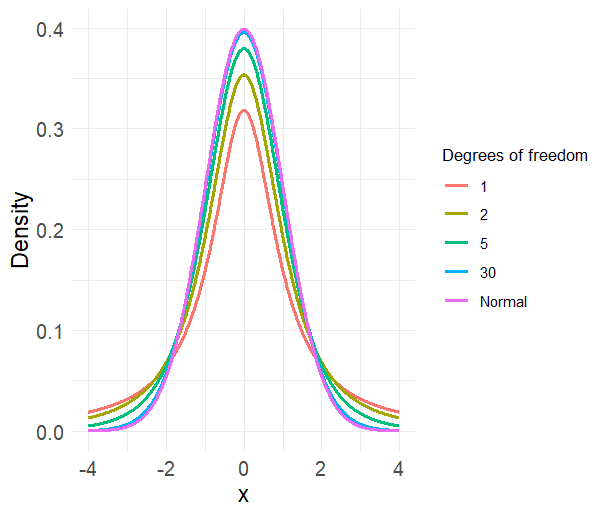
\includegraphics[width=\linewidth]{billder/T-distribution.png}
		\caption{The t-distribution as it approaches the standard normal distribution}
		\label{fig:t-dist}
	\end{minipage}\hfill
\end{figure}
